%!TEX root = ../dokumentation.tex
\chapter{Theoretische Hintergründe}

Vor dem Erstellen einer Schach-\acs{KI} (\acl{KI}) muss zunächst betrachtet werden, wie der Aufbau von KIs für spiel-mechanische Abläufe ist, welche Funktionen diese enthalten müssen und wie diese speziell auf das Spiel ``Schach'' angewandt werden können. Dazu werden zunächst Grundlagen der Spieltheorie betrachtet ehe näher auf Möglichkeiten zur Nutzung dieser im Kontext des Schachspiels eingegangen wird. Im zweiten Teil werden die verwendeten Methoden für die in dieser Arbeit beschriebene KI erläutert und die Wahl begründet.

\section{Spieltheorie}

\subsection{Geschichte}

Die Geschichte der Spieltheorie im Computerumfeld beginnt mit Claude Shannon im Jahre 1949, als dieser seine Gedanken zur möglichen Realisierung eines Schach spielenden Computers veröffentlicht. Dabei begründet er zunächst seine Auswahl auf das Spiel Schach für sein langfristiges Ziel eines spielenden Computers und legt dann das Ziel an sich fest.

\begin{quote}
“The chess machine is an ideal one to start with, since: (1) the problem is sharply defined both in allowed operations (the moves) and in the ultimate goal (checkmate); (2) it is neither so simple as to be trivial nor too difficult for satisfactory solution; (3) chess is generally considered to require ‘thinking’ for skillful play; a solution of this problem will force us either to admit the possibility of a mechanized thinking or to further restrict our concept of ‘thinking’; (4) the discrete structure of chess fits well into the digital nature of modern computers. … It is clear then that the problem is not that of designing a machine to play perfect chess (which is quite impractical) nor one which merely plays legal chess (which is trivial). We would like to play a skillful game, perhaps comparable to that of a good human player.”
\end{quote}

Die wesentlichen Punkte von Claude Shannon sind dabei, dass Schach weder zu simpel noch zu komplex ist, um es von einem Computer spielen zu lassen - Es gibt ein eindeutiges Ziel und eindeutige Operationen auf dem Weg zu diesem Ziel, aber kein eindeutig perfektes Spiel. Dementsprechend kann weder dies das Ziel sein, noch kann es das Ziel sein, einfach nur ein legales Spiel durchzuführen. Viel mehr muss es mit dem Schachspiel von Menschen vergleichbar sein. Menschen kennen den perfekten Zug nicht, können jedoch eine begrenzte Zahl an Zügen in dessen Wahrnehmungsbereich evaluieren und den in diesem Rahmen scheinbar besten Zug auswählen. Ein ähnliches Verhalten sollte auch bei einem Computer erkennbar sein.

Der vorgeschlagene Ansatz zum Evaluieren der Züge stellt dabei ein Algorithmus dar, der heute unter ``Minimax-Algorithmus'' bekannt ist. Dieser ruht auf dem ``Minimax-Theorem''  von John Vonn Neumann, der dieses 1929 beweisen konnte. Dieser Ansatz wird in Kapitel 2.1.2 erklärt.

Dieser Ansatz geht dabei davon aus, dass alle Spieler stets den optimalen Zug spielen. Das Ziel des Computers ist dabei alle möglichen Stati des Spiels zu berechnen, zu evaluieren und schlussendlich den Zug auszuwählen, der das voraussichtlich beste Endergebnis zur Folge hat. 

Dies ist für einen Computer leicht durchführbar. Dafür verlangt es folgende Informationen:
\begin{itemize}
\item Anfangszustand
\item Alle erreichbaren Zustände
\item Bewertung jedes einzelnen Zustandes
\end{itemize}

Um die erreichbaren Zustände zu erhalten, benötigt es einen Algorithmus, der an Hand der Spielregeln und eines Ausgangszustands s\textsubscript{0} alle erreichbaren Zustände nextStates berechnet. Von jedem Zustand enthalten in nextStates wird dann wiederum jeder mögliche erreichbare Zustand berechnet. Diese Schleife wird fortgeführt, bis die berechneten Zustände den Status eines Endzustandes erreichen, von dem aus keine Änderungen des Zustands mehr möglich sind.

Zudem braucht es eine Funktion, die die einzelnen Zustände evaluiert. Am Ende wird der Zug ausgewählt, der den erfolgreichsten Endzustand verspricht.

%http://www.andreykurenkov.com/writing/ai/a-brief-history-of-game-ai/

Dies ist solange umsetzbar, wie der Computer ohne Probleme alle möglichen Zustände berechnen und evaluieren kann. Um dies an einem Beispiel zu zeigen - Beim Spiel ``Tic Tac Toe'', bei dem in einem 3x3 Feld zwei Spieler gegeneinander antreten mit dem Ziel drei aneinander angrenzende (vertikal, horizontal oder diagonal) Felder mit ihrer Figur zu belegen, gibt es insgesamt 255.168 verschiedene Spielverläufe. Diese sind von heutigen Computern in akzeptabler Zeit berechenbar und evaluierbar.

%https://books.google.de/books?id=mUIzDwAAQBAJ&pg=PT18&lpg=PT18&dq=tic+tac+toe+m%C3%B6gliche+255+168&source=bl&ots=CcuZA068gP&sig=ACfU3U0XQ053sl4-BcVsL-hPnm76l1ZHyg&hl=de&sa=X&ved=2ahUKEwiL_snW6oLhAhXBIVAKHc7tD40Q6AEwAHoECAcQAQ#v=onepage&q=tic%20tac%20toe%20m%C3%B6gliche%20255%20168&f=false

Dazu bildet der Computer einen Minimax-Baum, wie in Kapitel 2.1.2 beschrieben, und wählt dann den erfolgversprechendsten Zug aus. Nach jedem getätigten Zug werden die erreichbaren Zustände nur noch vom neuen Zustand aus berechnet. Im Spätspiel kann dies bei ``Tic Tac Toe'' beispielsweise aussehen wie in Figur 2.1.1.1

\begin{figure}[h]
\centering
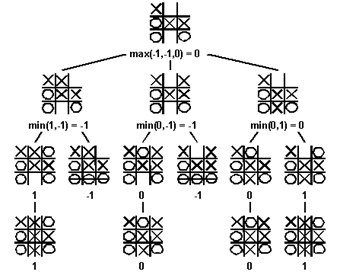
\includegraphics[width=\textwidth/5*3]{images/tictactoe_minimax_tree.png}

\textsuperscript{Figure 2.1.1.1 Tic Tac Toe Minimax Baum \cite{}}\\
\end{figure}
%http://www.andreykurenkov.com/writing/ai/a-brief-history-of-game-ai/

Dabei werden vom Ausgangszustand, der den Zustand des aktuellen Spiels widerspiegelt, aus alle möglichen Folgezustände berechnet. Von diesen werden wiederum alle möglichen Folgezustände berechnet. Dies wird solange fortgeführt, bis alle neu berechneten Zustände Endzustände sind. Dann werden alle Endzustände evaluiert. Eine 1 stellt dabei einen Sieg dar, eine 0 ein Unentschieden und eine -1 eine Niederlage. Da davon ausgegangen wird, dass der gegnerische Spieler stets den besten Zug auswählt, wird jeder Zustand, der noch Folgezustände besitzt, mit dem für ihn schlechtesten Wert aller seiner möglichen Folgezustände bewertet. Der Computer wählt dann den Zustand mit der für ihn besten Bewertung.
%zu minimax?

In diesem Beispiel wird sich der Computer somit für den dritten Zug von links entscheiden, da bei beiden anderen ein Sieg des Gegenspielers bevorsteht, sollte dieser jeweils die perfekten Züge spielen. Beim dritten Zug kann der Gegner maximal noch ein Unentschieden erreichen.

Diese Strategie gerät jedoch dann an ihre Grenzen, wenn nicht mehr alle möglichen Zustände berechnet werden können. Bei dem Spiel Schach beispielsweise belaufen sich Schätzungen schon nach den ersten 40 Spielzügen auf 10\textsuperscript{115} - 10\textsuperscript{120} verschiedene Spielverläufe. Dies ist auch für einen Computer in tolerierbarer  Zeit unmöglich berechenbar. Aus diesem Grund muss die Strategie für solch komplexere Spiele abgewandelt werden. Die verschiedenen Ansätze dazu sind in Kapitel 2.1.3 beschrieben.

% Eero Bonsdorff, Karl Fabel, Olavi Riihimaa: Schach und Zahl. 3. Auflage, Rau, Düsseldorf 1978.
%https://de.wikipedia.org/wiki/Schach#cite_note-6


\subsection{Minimax-Algorithmus}


\subsection{Problematik Minimax-Algorithmen komplexerer Spiele}



% Einleitung: Alle Züge evaluierbar
% Evaluerungsmöglichkeiten
   % board wert (Figuren)
   % attackierte figuren
   % board wert (Figuren + Positionen)
   % History
   % Wichtige Figuren attackierbar => ---
   % abrubtes ende wenn bestimmter zug spiel beendet (finishing - wenn bauer zu schlagen spiel beendet dann sollte man das machen)
% Überleitung: Nicht mehr alle evaluierbar => Iterative Deepening
% Methoden: Bestimmte Tiefe / Bestimmte Zeit
% Minimax
%Improvement: Alpha Beta
% Opening book
   % wozu
% Finishing book/strategy?
   % wozu (ewige jagd; attackierte figur von einer seite genauso viel wert wie von mehreren seiten)
   
   
% andere attackierte figuren evaluation?
% defense evaluation
% controlling evaluation?



\section{Verwendete Methoden}
- Ealuierungsfunktionen - weiß + schwarz -
- Minimax/alpha beta
